\chapter{Virtuelle Klassenzimmer}

\section{Definition}
Übersetzt man E-Learning aus dem englischen in das deutsche kann darunter  \glqq elektronisches Lernen\grqq{} oder \glqq computergestütztes Lernen\grqq{} verstanden werden. Eine andere Definition ist \glqq das Lehren und Lernen mit Hilfe verschiedener elektronischer Medien\grqq{} \cite[vgl.][]{elearning}. \newline
\newline Weiterhin wird versucht durch verschiedene Klassifizierungen den Begriff zu umschreiben. Darunter fallen die Interaktivität, Multicodalität, Multimedialität und Multimodalität.

\subsection{Interaktivität} 
		 Interaktiv bedeutet, dass der Benutzer verschiedenen Möglichkeiten hat Einzugreifen oder zu Steuern. Einfachste Interaktionen sind bspw. das Stoppen von Videos und das Vor- Zurückspulen dieser. Die höchste Form der Interaktivität ist, eine Präsentation mit anschliessendem Feedback und Diskussionsrunde \cite[vgl.][]{elearning.interaktivitaet}. 
\subsection{Multicodalität}
		 Hierbei geht es um die Darbietungsart der Information. Beispielsweise als Bild, Text und Animation. Als neuste Form kommen die Simulationen dabei in die Betrachtung. Hier kann der Lernende virtuelle Experimente, Berechnungen, etc. durchführen und meisten grafisch anzeigen lassen.  \cite[vgl.][]{elearning.multicodalitaet2}. 
\subsection{Multimedialität}
		 Multimedialität meint, die verschiedenen Möglichkeiten wie die Medien dargeboten werden. Verschiedene Medien können beispielsweise Bücher, Videoplayer, Audioplayer, Computer, Hörbücher, E-Books sein.  \cite[vgl.][]{elearning.multimedialitaet2}. \newline  \newline
\subsection{Multimodalität}
		 Unter der Multimodalität versteh sich die Aufnahme und Verarbeitung  von Informationen über die verschiedenen Sinne des Menschen. Hauptsächlich betrifft dies die auditiven und visuellen Sinne.  \cite[vgl.][]{elearning.multimodalitaet}. 

\section{Entwicklung}
Den Lehr- und Lernprozess elektronisch zu unterstützen, ist eine zeitgemässe Weiterentwicklung \cite[vgl.][S.5]{Dittler}. Schon Mitte der 60er Jahre war die Entwicklung von computerbasierten Unterrichtsmaschinen in der Lehre im Einsatz. Durch Texte mit Audios, Bildern und auch Filmen wurde diese unterstützt \cite[vgl.][S.12]{Dittler}. In den späten 90er Jahren entwickelten sich der Einsatz von hochwertigeren Video- und Audiosequenzen weiter. Durch die Verfügbarkeit von Internet, waren Web-Based-Trainings (WBT) möglich. Sie unterscheiden sich von Computer-Based-Trainings technisch. Da bedeutet, dass bei WBT keine CDs oder Disketten mehr nötig waren. Mit WBT konnten an die Lernenden die URL versendet werden, wo sie dann den Zugriff auf die Anwendung erhielten \cite[vgl.][S.23]{Dittler}. Die Entwicklungen zwischen 2005 und 2012 zielten auf den „User-Generated Content“ ab. Darunter fallen Blogs, Wikis und Podcasts. Diese neuen Kommunikationsformen ergänzen das WBT hinsichtlich des Austauschens in Form von geteilten Meinungen, Erfahrungen und Eindrücken. \cite[vgl.][S.31]{Dittler}. Seit den 200er spielen Smart Devices, wie z.B. Smartphones, Tablets und Laptops, welche in nahezu allen Haushalten zur Verfügung stehen, eine immense Rolle des täglichen Ablaufs. Das bedeutet, dass der Lernprozess sich im Bereiche Lernort, Lernzeitpunkt und Lernform aus dem traditionellen Blickwinkel, z.B. zum klassische Buch und Schulunterricht, stark verändern kann und teilweise schon hat \cite[vgl.][S.51]{Dittler}. 

\section{Mixed Reality}

\subsection{Definition}
Die wörtlich übersetzte „gemischte Realität“ ist eine Fusion zwischen der physischen und digitalen Welt. Durch Fortschritte in der Forschung von Grafikleistung, Computer Vision, Displaytechnologie und Eingabesystemen wird dies ermöglicht. Der Begriff Mixed Reality wurde von Paul Milgram und Fumio Kishino in ihrem Paper „A Taxonomy of Mixed Reality Visual Displays.“ 1994 erstmals erwähnt. 
In den letzten Jahrzehnten wurde die Input-Beziehung von Menschen und Computern gut erforscht. Es besteht eine weit verbreitete Disziplin, die als Human Computer Interaction oder HCI bekannt ist. Menschlicher Input, oder auch Eingaben genannt, erfolgen über eine Vielzahl von Mitteln, darunter Tastaturen, Mäuse, Touch, Stimme und sogar Kinect-Skelett-Tracking.
Fortschritte in der Sensorik und Verarbeitung führen zu neuen Möglichkeiten in dem Bereich Computer Input. Die Interaktionen zwischen Computer und Umgebung werden effektiver beim Umweltverständnis und der Wahrnehmung. Daher werden die API-Namen in Windows, die Umweltinformationen enthalten, als Wahrnehmungs-APIs bezeichnet. Umwelteinflüsse erfassen Dinge wie die Position einer Person in der Welt (z.B. Kopfverfolgung), Oberflächen und Grenzen (z.B. räumliche Kartierung und räumliches Verständnis), Umgebungsbeleuchtung, Umgebungsgeräusche, Objekterkennung und Ortung.
Jetzt bietet die Kombination aller drei - Computerverarbeitung, menschlicher Input und Umwelteinfluss - die Möglichkeit, echte Mixed-Reality-Erlebnisse zu schaffen. Bewegung durch die physische Welt kann zu Bewegung in der digitalen Welt führen. Grenzen in der physischen Welt können Anwendungserfahrungen, wie z.B. das Spielen von Spielen, in der digitalen Welt beeinflussen. Ohne Umwelteinfluss könnten Erfahrungen nicht zwischen der physischen und der digitalen Realität verschmelzen.

\begin{figure}[ht]
	\centering
	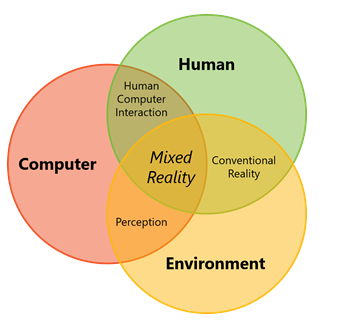
\includegraphics[width=\textwidth,height=\textheight,keepaspectratio]{images/venndiagramm.png}
	\caption{Mixed-Reality \\ Quelle: \cite[vgl.][]{BrandonBray}}
	\label{Mixed-Reality4}
\end{figure}

\subsection{Spektrum}
Da die Mixed-Reality die Verschmelzung von physischer und digitaler Welt ist, definieren diese beiden Realitäten die polaren Enden eines Spektrums, das als Virtualitätskontinuum bekannt ist. Genannt wir dies das Mixed-Reality-Spektrum. Auf der linken Seite haben wir die physische Realität, in der wir, die Menschen, leben. Dann haben wir auf der rechten Seite die entsprechende digitale Realität.

\begin{figure}[ht]
	\centering
	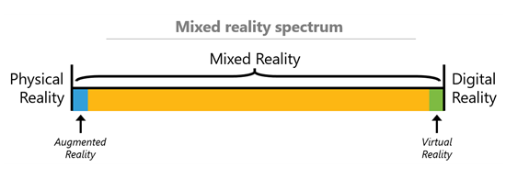
\includegraphics[width=\textwidth,height=\textheight,keepaspectratio]{images/MixedRealitySpektrum.png}
	\caption{Mixed-Reality-Spektrum \\ Quelle: \cite[vgl.][]{BrandonBray}}
	\label{Mixed-Reality3}
\end{figure}

Die meisten Mobiltelefone auf dem Markt haben heute wenig bis gar kein Umweltverständnis. Die Erfahrungen, die sie bieten, können sich also nicht zwischen physischen und digitalen Realitäten vermischen. Die Erfahrungen, die Grafiken auf Videostreams der physischen Welt überlagern, sind Augmented Reality, und die Erfahrungen, die den Blick auf eine digitale Erfahrung versperren, sind Virtual Reality. Die meisten heute verfügbaren Augmented Reality und Virtual Reality Angebote stellen einen sehr kleinen Teil dieses Spektrums dar. Sie sind jedoch Teilmengen des größeren Mixed-Reality-Spektrums. \newline 

\noindent Es gibt zwei Haupttypen von Geräten, die Mixed Reality-Erlebnisse bieten:
\begin{enumerate}[leftmargin=*,label= \arabic*:]
	 \item Holographische Geräte: Diese zeichnen sich durch die Fähigkeit des Geräts aus, digitale Inhalte in der realen Welt so zu platzieren, als ob sie wirklich vorhanden wären. 
	  \item Immersive Geräte. Diese zeichnen sich durch die Fähigkeit des Gerätes aus, ein Gefühl von „Präsenz“ zu erzeugen - die physische Welt zu verbergen und durch ein digitales Erlebnis zu ersetzen.
\end{enumerate}

\begin{figure}[ht]
	\centering
	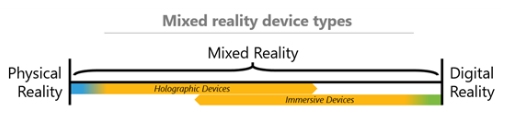
\includegraphics[width=\textwidth,height=\textheight,keepaspectratio]{images/MixedRealityDeviceTypes.png}
	\caption{Mixed Reality Device Types \\ Quelle: \cite[vgl.][]{BrandonBray}}
	\label{Mixed-Reality2}
\end{figure}

\section{Endgeräte}

Es gibt heute keine Geräte, die das gesamte Spektrum abdecken können, aber in Zukunft werden holographische Geräte immer mehr und immersive Geräte immer mehr holographisch werden.
\begin{itemize}
	\item Nach links (nahe der physischen Realität). Benutzer bleiben in ihrer physischen Umgebung präsent und werden nie zu dem Schluss gebracht, dass sie diese Umgebung verlassen haben.
	\item In der Mitte (vollständig gemischte Realität). Diese Erfahrungen verbinden die reale und die digitale Welt perfekt. Zuschauer, die den Film Jumanji gesehen haben, können verstehen, wie die physische Struktur des Hauses, in dem die Geschichte stattfand, mit einer Dschungelumgebung vermischt wurde.
	\item Nach rechts (nahe der digitalen Realität). Die Benutzer erleben eine vollständig digitale Umgebung und wissen nicht, was in der physischen Umgebung um sie herum geschieht.
\end{itemize}

\begin{figure}[ht]
	\centering
	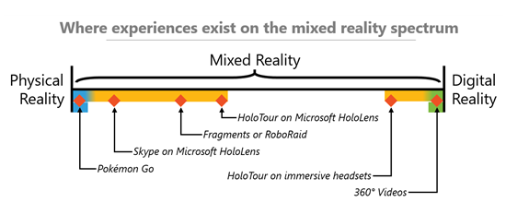
\includegraphics[width=\textwidth,height=\textheight,keepaspectratio]{images/BeispielemitMixedReality.png}
	\caption{Beispiele mit Mixed-Reality \\ Quelle: \cite[vgl.][]{BrandonBray}}
	\label{Mixed-Reality1}
\end{figure}

	
Es gibt unterschiedliche Möglichkeiten im Mixed-Reality-Spektrum:
\begin{description}
	\item . 
	\begin{itemize}
		\item Skype auf Microsoft HoloLens. Diese Erfahrung ermöglicht die Zusammenarbeit durch das Zeichnen in der physischen Umgebung. Als eine Erfahrung, ist es derzeit weiter auf dem Spektrum links, weil die physische Umgebung der Ort der Aktivität bleibt.
		\item Fragmente und RoboRaid. Beide nutzen das Layout der physischen Umgebung des Nutzers, Wände, Böden und Möbel, um digitale Inhalte in der Welt zu platzieren. Die Erfahrung bewegt sich weiter nach rechts auf dem Spektrum, aber der Benutzer glaubt immer, dass er sich in seiner physischen Welt befindet.
		\item HoloTour auf immersiven Geräten. HoloTour ist für ein immersives Erlebnis konzipiert. Die Benutzer sind dazu bestimmt, an touristischen Orten herumzulaufen. Die Grenzen, die dem Benutzer helfen, das Betreten von Wänden zu vermeiden, stellen weitere Fähigkeiten dar, die das Erlebnis in die Mitte ziehen.
		\item 360 Grad-Videos. Da Umwelteinflüsse wie Translationsbewegungen das Video-Wiedergabe-Erlebnis nicht beeinflussen, fallen diese Erfahrungen ganz nach rechts in die digitale Realität und fügen sich in den engen Bereich des Spektrums der virtuellen Realität ein \cite[vgl.][]{BrandonBray}.
		\item  Immersive Bildung mit der HoloLens. Das Start-Up Unternehmen Lifeliqe ist in einer Partnerschafft mit Microsoft und rückt das Lernen in der Mixed-Rality in den Vordergrund. Sie führten Pilot-Unterrichtsstunden mit der HoloLens an der Renton Prep in Seattle, Washington, und dem Castro Valley Unified College in Californien durch. Durch interaktive 3D-Modelle des menschlichen Körpers mit samt seinen Orangen, Blutzellen und Knochen, konnten die Schüler diesen mit der Microsoft HoloLens erkunden \cite[vgl.][]{vrnerds.2017}. 
	\end{itemize}
\end{description}


\section{HTC Vive}
Die HTC Vive ist eine VR Brille die von HTC in Kooperation mit Valve produziert wurde. In San Francisco an der Alta Vista Schule ist diese im Einsatz. In der Lifeliqe VR Museum App können die Schüler virtuell durch Ruinen wandern, Zellen von Lebewesen genau betrachten oder im Weltall schweben. So lernen die Schüler auf eine spielerische Art und Weise auch anspruchsvollere wissenschaftliche Themen zu handhaben. Die HTC Vive ermöglicht eine interaktive Lernerfahrung. Durch Bewegungen ermöglicht es den Schülern ein Gefühl der Kontrolle zu erlangen, was den Lernprozess in Bezug auf Selbstbewusstsein stärkt  \cite[vgl.][]{vrnerds2.2017}.

\section{Visuelle Anwesenheit}
Das virtuelle Klassenzimmer ermöglicht es, das die Schüler von zu Hause aus am Unterricht teilnehmen können. In Australien ist dies schon lange im Einsatz, da teilweise die nächste Schule mehrerer hunderte Kilometer entfernt liegt. Solange alle Schüler das gleiche sehen, hören und erleben können wie wen sie im Klassenzimmer anwesend währen, Ist ein synchroner Unterricht gegeben. Die lernenden sollen miteinander kommunizieren können und auch in der Lage sein Daten auszutauschen \cite[vgl.][]{mikogo.2010}. \pagebreak

\noindent Die Moderation kann auf unterschiedliche Weise erfolgen. 

	\begin{itemize}
		\item Dozentengeführter Modus: Der Lehrer oder Dozent hat eine größere Gruppe zu betreuen und ist daher in der Lage zu entscheiden welche Wortmeldung er erteilen will. Das ist dazu gedacht, dass in großen Gruppen kein Stimmen Wirrwarr entsteht. 
		\item Offen Diskussionen: Ist in dem Fall genau das Gegenteil. Jeder Schüler hat die Möglichkeit per Mausklick sich zu Wort zu melden. Diese Variante eignet sich für kleine Gruppen.
		\item Arbeitsgruppen: Hier unterteilt man für bestimmte Aufgaben die große Gruppe in kleine Gruppen und erteilt ihnen die offene Diskussion als Moderationsweg
		\item Co-Moderation: Eignet sich dann, wenn zusätzliche Dozenten, Lehrer beteiligt werden sollen an der Unterrichtsstunde. Beispielsweise kann ein Experte der Physik aus den USA zugeschalten werden und mit den Rechten des Dozentengeführten Modus ausgestattet werden. So kann er auf einzelne Fragen eingehen ohne unterbrochen zu werden von seinem Vortrag. Der Lehrer wiederum kann sich im Fall dazwischen schalten \cite[vgl.][]{managementcircle.de.2017}.
	\end{itemize}

\section{BYOD}
Ausgeschrieben bedeutet BYOD, Bring Your Own Device und übersetzt, bring dein eigenes Endgerät mit. Da nahezu jeder Schüler zwischen 12 und 19 Jahren mittlerweile ein Smartphone mit Datenflatrate besitzt, ca. 92 \%, lässt sich dies in den Unterricht leicht integrieren. Gerade für den VR Ansatz spielt das eine große Rolle. Für die paar wenigen Schüler die kein Smartphone oder Tablett besitzen könnte die Schule Leihgeräte anschaffen und die Kosten würden somit nicht exorbitant steigen. Die Flatrate Thematik könnte in den nächsten Jahren hinfällig werden, wenn alle Schulen ihr WLAN zur Verfügung stellen. Bis dahin müssten die paar wenigen Schüler die keine Flatrate besitzen die Kosten bei der Schule einreichen für den zusätzlichen Datenverbrauch \cite[vgl.][]{Cardboard1}. 
Eine günstige Alternative zu den teuren VR Brillen die es im Angebot gibt, ist die Google Cardboard. Diese Variante wird selbst zusammen gebastelt und kosten ca. 14 \euro{}. Man legt sein Smartphone in den Karton und legt die Brille mit Gummibändern an den Kopf an. Durch passende Apps dazu die heruntergeladen werden müssen kann das VR Erlebnis beginnen \cite[vgl.][]{Cardboard2}.

\begin{figure}[ht]
	\centering
	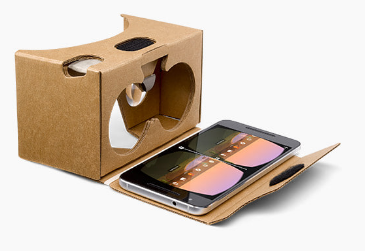
\includegraphics[width=\textwidth,height=\textheight,keepaspectratio]{images/GoogleCarboard.png}
	\caption{Google Cardboard  \\ Quelle: \cite[vgl.][]{Cardboard2}}
	\label{Google Cardboard}
\end{figure}

\section{Studie zu VR im Unterricht}
Abschliessen bestätigt die Studie “A Case Study - The Impact of VR on Academic Performance” der Beijing Bluefocus E-Commerce Co., Ltd. und Beijing iBokan Wisdom Mobile Internet Technology Training Institutions die Vorteile von VR Lernen. In der Studie wurden Schüler in zwei Gruppen geteilt. Die eine Gruppe lernte weiterhin traditionell mit Büchern und die andere mit VR. Die Testgruppe die mit VR lernen durfte erreicht einen Zielwert von 93 Punkten und die Bücher Gruppe von nur 73 Punkten  \cite[vgl.][]{htcvive}.

\begin{figure}[ht]
	\centering
	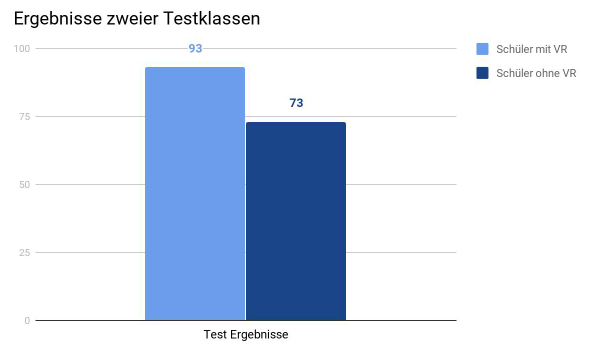
\includegraphics[width=\textwidth,height=\textheight,keepaspectratio]{images/TestergebnisseGruppen.png}
	\caption{Testergebnisse zweier Gruppen \\ Quelle: \cite[vgl.][]{htcvive}}
	\label{Testergebnisse zweier Gruppen}
\end{figure}

\begin{figure}[ht]
	\centering
	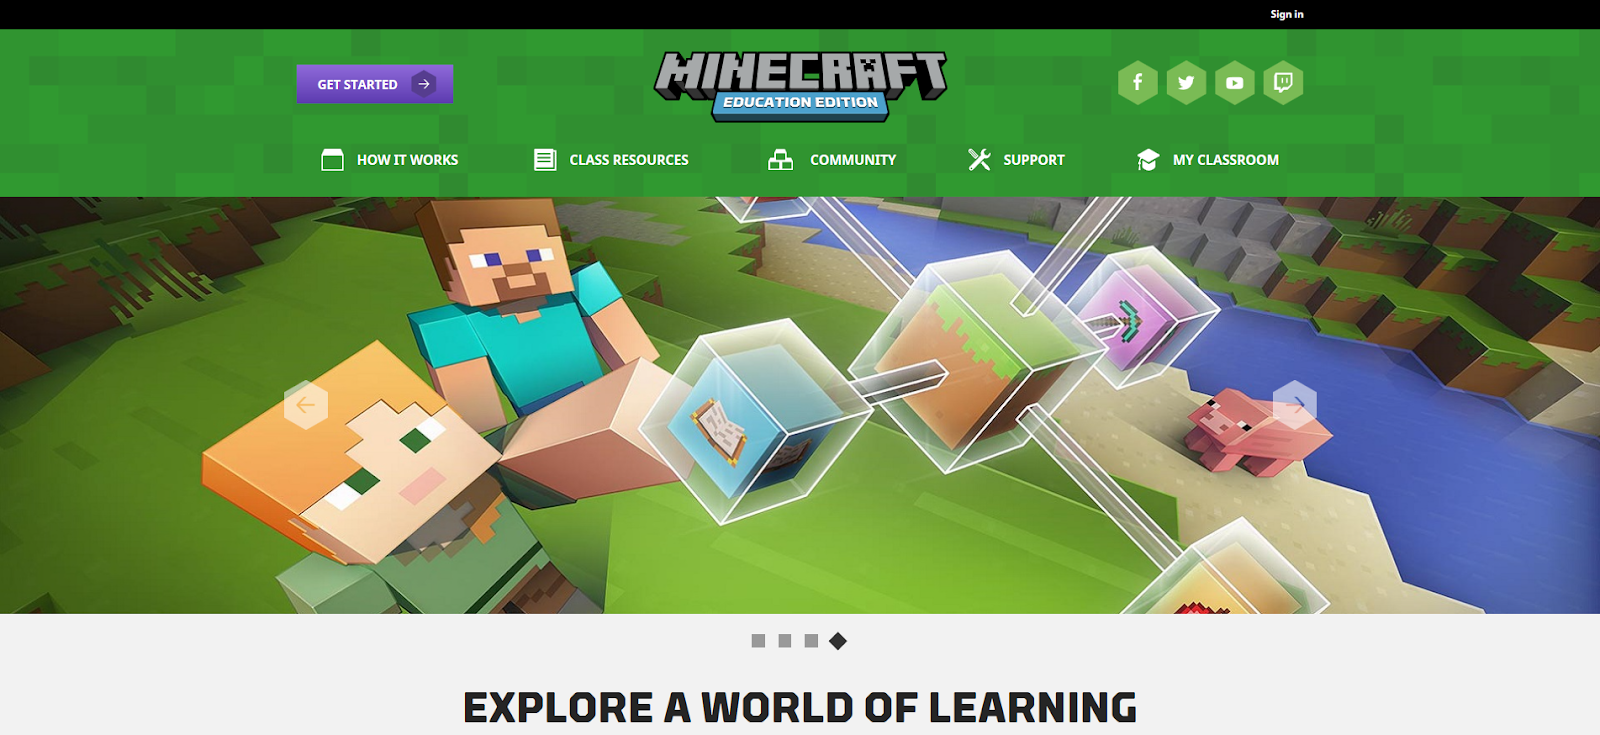
\includegraphics[width=\textwidth,height=\textheight,keepaspectratio]{images/Minecraft.png}
	\caption{Projekt Minecraft in Education \cite{HomepageMinecraftEducation}}
	\label{projectMinecraft}
\end{figure}

\section{Fazit}
Wie in der soeben vorgestellten Studie erwähnt, kann VR im Unterricht zu neuen Leistungszielen helfen. Die Schüler bekommen neue Lernarten vorgestellt und können interaktiv sich Wissen aneignen. VR muss die Kosten von Schulen nicht in die Höhe treiben wen man auf bspw. Die Google Cardboard zurückgreift und die Smartphones der Schüler einsetzt. Über den Datenschutz und Sicherheitskonzepte bei Prüfungen kann und muss noch tiefer diskutiert werden, was aber hier in der vorliegenden Arbeit kein Bestandteil war. Die vorgestellten Beispiele für die VR-Brillen zielten auf Lernstoff ab, welcher auch gut durch Visuelle Reize zu verarbeiten ist, wie bspw. Biologie, Geschichte, Chemie etc. Allerdings können immer mehr Schulfächer integriert werden wie Sprachen, Politik, Wirtschaft, usw. Für das virtuelle Klassenzimmer kommt jedes Fach in Frage. 
Es bleibt abzuwarten welche weitere Trends und Umsetzungen daraus resultieren werden und wie schnell Schulen und andere Institutionen diese adaptieren können. 